% kuleuventheme2 by Janez Kren, September 2017, janez.kren@kuleuven.be, based on:
% kuleuventheme 1.3 by Roland Pastorino, 2013 roland.pastorino@kuleuven.be / www.rolandpastorino.com

\documentclass[11pt,t]{beamer}
\usetheme{kuleuven2}	%THEME OPTIONS for LOGO: kul (default), kulak, lrd,    ; OPTIONS for TITLE PAGE: normal (default), sedes


%%% OTHER SETTINGS
\usefonttheme[onlymath]{serif}			% math font with serifs, delete to make it sans-serif
\setbeamertemplate{footline}[body] 		% delete this line to remove footline bar on all frames
\usepackage[orientation=landscape,size=custom,width=16,height=9,scale=0.5,debug]{beamerposter} %enable for widescreen 16:9 ratio
%\titlegraphic{ \includegraphics[width=.2\paperwidth]{mytitlepagepic.png} } %optional title page image


%%% ADDED PACKAGES:
\usepackage[english]{babel}
\usepackage{amsfonts}
\usepackage{amssymb}
\usepackage{mathtools}
\usepackage{graphicx}

\graphicspath{{images/}} 

\newcommand{\Int}{\int\limits}


%%% TITLE PAGE INFO:
\title[]{High-Performance Numerical Simulation of Biodegradation Process with Moving Boundaries} %[] will appear in footline
\subtitle{FreeFEM Days, 11th Edition}

\author{Mojtaba Barzegari, Liesbet Geris}
\institute{Biomechanics Section, Department of Mechanical Engineering, KU Leuven}
\date{December 2019}




\begin{document}
\csname beamer@calculateheadfoot\endcsname %recalculate head and foot dimension

% Title page
\begin{frame}[plain,noframenumbering]
	\titlepage
\end{frame}
	
%
%% Table of Contents
%\begin{frame}{Outline}
%			\setstretch{0.6}
%	\hfill	{\large \parbox{.961\textwidth}{\tableofcontents[hideothersubsections]}}
%\end{frame}

\begin{frame}[fragile]{Our Research Group}  


\begin{itemize}
\item
Supervisor: Prof. Ir. Liesbet Geris
\item
Research profile:
\\
Computational Tissue Engineering, Computational Biomechanics, Computational Biology, Computational Genomics
\end{itemize}

	\begin{figure}
			\centering
			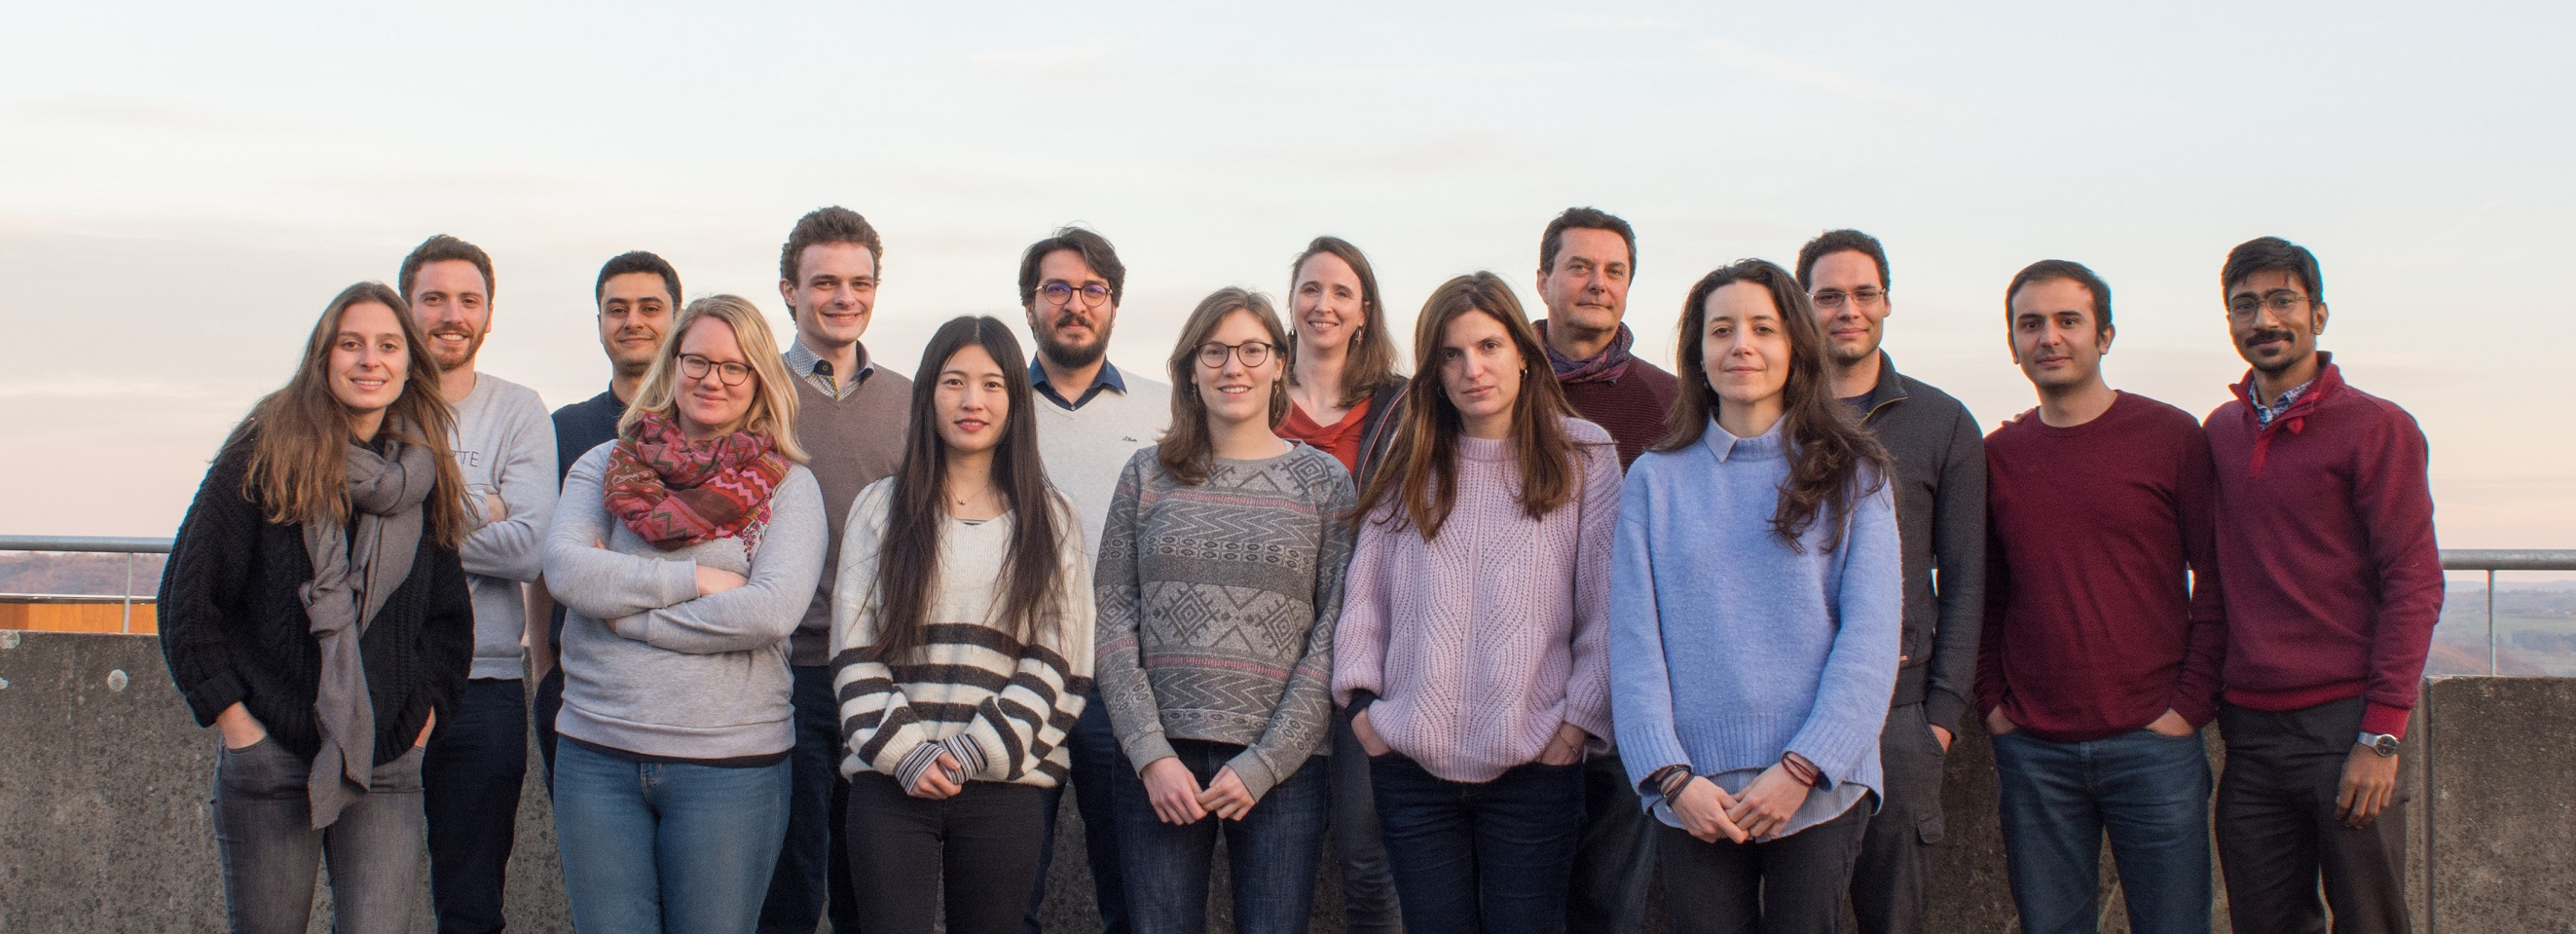
\includegraphics[width=0.74\textwidth]{team}
			 
	\end{figure}

\end{frame}


\section{Introduction}

\begin{frame}[fragile]{Reaction-Diffusion Systems with Moving Boundaries}  

\begin{itemize}
\item
Stefan problems
\item
Diffusion-controlled interface
\item
 Diffusion and reaction lead to the change of domain geometry
 \item 
 Degradation is an example of such a system
\end{itemize}

\end{frame}


\begin{frame}[fragile]{Biodegradation Process}  

\begin{itemize}
\item
Dissolution of the bulk material 
\item
Formation of a protective film
\item
 Effect of ions in the medium
\end{itemize}

	\begin{figure}
			\centering
			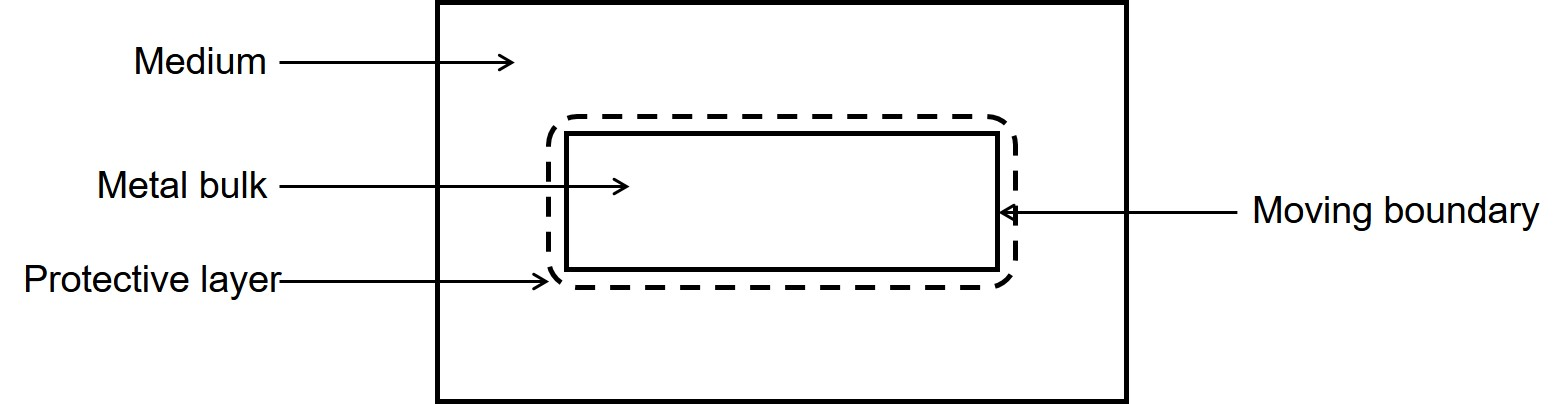
\includegraphics[width=0.85\textwidth]{schematic}
			 
	\end{figure}

\end{frame}


\begin{frame}[fragile]{A Sample Application}  

\begin{itemize}
\item
Hip joint replacement implants
\item
Tuning the degradation parameters to the rate of bone growth
\end{itemize}

\vspace{0.5cm}
	\begin{figure}
			\centering
			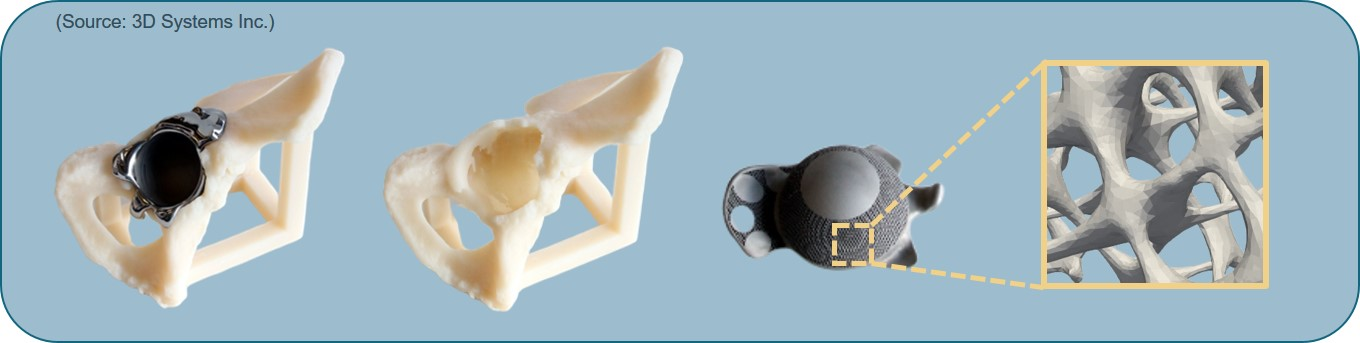
\includegraphics[width=0.9\textwidth]{hip_implant}
			 
	\end{figure}

\end{frame}


\section{Mathematical Model}


\begin{frame}[fragile]{Chemistry of Biodegradation}


	\begin{columns}[t]
		\begin{column}{.5\textwidth}
Some of the chemical reactions:
\begin{gather*}
\mathrm{Mg} \rightarrow \mathrm{Mg}^{2+}+2 \mathrm{e}^{-}
\end{gather*}
\begin{gather*}
2 \mathrm{H}_{2} \mathrm{O}+2 \mathrm{e}^{-} \rightarrow \mathrm{H}_{2}+2 \mathrm{OH}^{-}
\end{gather*}
\begin{gather*}
\mathrm{Mg}^{2+}+2 \mathrm{OH}^{-} \xrightarrow{k_1} \mathrm{Mg}(\mathrm{OH})_{2}
\end{gather*}
\begin{gather*}
\mathrm{Mg}(\mathrm{OH})_{2}+2\mathrm{Cl}^{-} \xrightarrow{k_2} \mathrm{Mg}^{2+} + 2\mathrm{Cl}^{-} + 2\mathrm{OH}^{-}
\end{gather*}
		\end{column}
		\begin{column}{.5\textwidth}

			\begin{figure}
			\centering
			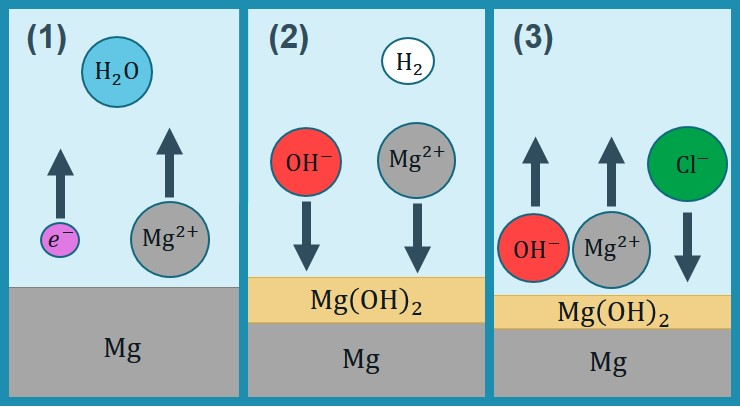
\includegraphics[width=\textwidth]{chemistry}
			 
			\end{figure}
		\end{column}
	\end{columns}

\end{frame}


\begin{frame}[fragile]{Reaction-Diffusion Equations}

\vspace{-0.8cm}


\begin{gather*}
C_{\mathrm{Mg}} = C_{\mathrm{Mg}}(x,t), \quad C_{\mathrm{Film}} = C_{\mathrm{Film}}(x,t) \quad x \in \Omega \subset \mathbb{R}^{3}
\end{gather*}
\begin{gather*}
\frac{\partial C_{\mathrm{Mg}}}{\partial t}=\nabla \bullet \left(D_{\mathrm{Mg}}^{e} \bullet  \nabla C_{\mathrm{Mg}} \right)-k_{1} C_{\mathrm{Mg}}\left(1-\frac{C_{\mathrm{Film}}}{[\mathrm{Film}]_{\max }}\right) +k_{2} C_{\mathrm{Film}} [\mathrm{Cl}]^{2}
\end{gather*}
\begin{gather*}
\frac{\partial C_\mathrm{Film}}{\partial t}=k_{1} C_{\mathrm{Mg}}\left(1-\frac{C_{\mathrm{Film}}}{[\mathrm{Film}]_{\max }}\right) -k_{2} C_{\mathrm{Film}} [\mathrm{Cl}]^{2}
\end{gather*}
\begin{gather*}
D_{\mathrm{Mg}}^{e}=D_{\mathrm{Mg}}\left(\left(1-\frac{C_{\mathrm{Film}}}{[\mathrm{Film}]_{\max }}\right)+\frac{C_{\mathrm{Film}}}{[\mathrm{Film}]_{\max }} \frac{\epsilon}{\tau}\right)
\end{gather*}

\end{frame}


\begin{frame}[fragile]{Level Set Method}  

Implicit signed distance function  $\phi = \phi(x,t) \quad x \in \Omega \subset \mathbb{R}^{3}$
\begin{gather*} \label{eq:lsm_full}
\frac{\partial \phi}{\partial t}+\underbrace{\overrightarrow{V} \bullet \nabla \phi}_{\text {External velocity field }}+\underbrace{\mathrm{v}|\nabla \phi|}_{\text {Normal direction motion }}=\underbrace{b \kappa|\nabla \phi|}_{\text {Curvature - dependent term }}
\end{gather*}


	\begin{figure}
			\centering
			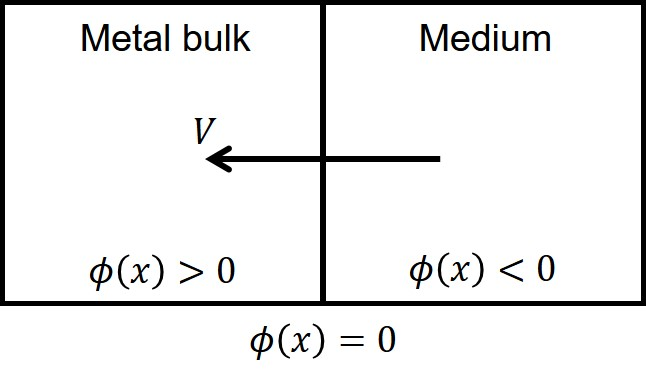
\includegraphics[width=0.4\textwidth]{level_set_domain}
			 
	\end{figure}

\end{frame}

\begin{frame}[fragile]{Coupling Mass Transfer and Level Set}

	\begin{columns}[t]
		\begin{column}{.6\textwidth}
		\vspace{-0.7cm}
		\begin{gather*}
		\frac{\partial \phi}{\partial t}+\mathrm{v}|\nabla \phi|=0
		\end{gather*}
Rankine-Hugoniot:
		\begin{gather*}
		\left\{\mathbf{J}(x, t)-\left(c_{\mathrm{sol}}-c_{\mathrm{sat}}\right) \mathrm{v}(x, t)\right\} \cdot n=0
		\end{gather*}
		\begin{gather*}
		D_{\mathrm{Mg}}^{e} \nabla_{n} C_\mathrm{Mg}-\left([\mathrm{Mg}]_{\mathrm{sol}}-[\mathrm{Mg}]_{\mathrm{sat}}\right) \mathrm{v}=0
		\end{gather*}		
		\begin{gather*}
\frac{\partial \phi}{\partial t}-\frac{D_{\mathrm{Mg}}^{e} \nabla_{n} C_\mathrm{Mg}}{[\mathrm{Mg}]_{\mathrm{sol}}-[\mathrm{Mg}]_{\mathrm{sat}}}|\nabla \phi|=0
		\end{gather*}		
		
		
		
		\end{column}
		\begin{column}{.4\textwidth}
			\vspace{-0.8cm}
			\begin{figure}
			\centering
			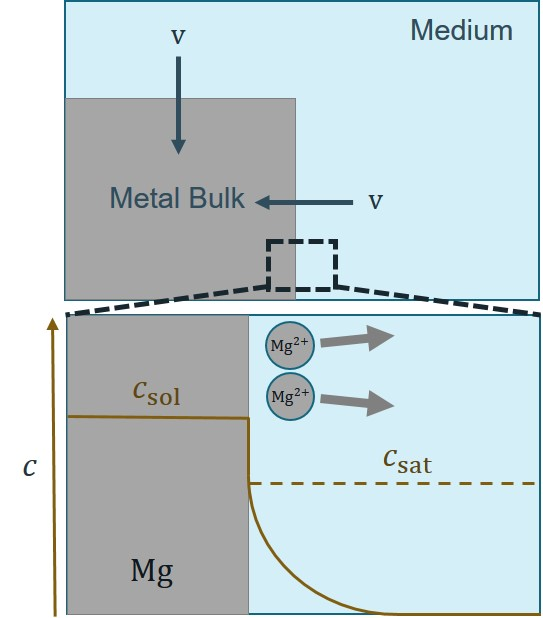
\includegraphics[width=\textwidth]{rankine}
			 
			\end{figure}
		\end{column}
	\end{columns}

\end{frame}


\section{Computational Model and Parallelization}

\begin{frame}[fragile]{Weak Formulation}

Rewriting the diffusion-reaction PDE:
\begin{gather*}
\frac{\partial u}{\partial t}=\nabla \bullet (D \bullet  \nabla u)-k_{1} a u+k_{2} p q^{2}
\end{gather*}

Defining trial and test function space:
\begin{gather*}
\mathcal{S}_{t}=\left\{u(\mathbf{x}, t) | \mathbf{x} \in \Omega, t>0, u(\mathbf{x}, t) \in \mathcal{H}^{1}(\Omega), \text { and } \frac{\partial u}{\partial n}=0 \text { on } \Gamma\right\}
\end{gather*}
\begin{gather*}
\mathcal{V}=\left\{v(\mathbf{x}) | \mathbf{x} \in {\Omega}, v(\mathbf{x}) \in \mathcal{H}^{1}(\Omega), \text { and } v(\mathbf{x})=0 \text { on } \Gamma\right\}
\end{gather*}


\end{frame}


\begin{frame}[fragile]{Weak Formulation cont.}

\begin{gather*}
\frac{\partial u}{\partial t} v=\nabla \bullet (D \bullet \nabla u) v-k_{1} b u v+k_{2} p q^{2} v \quad \forall v \in \mathcal{V}
\end{gather*}
Integrate over the whole domain:
\begin{gather*}
\int_{\Omega} \frac{\partial u}{\partial t} v d \omega=\int_{\Omega} \nabla \bullet (D \bullet \nabla u) v d \omega-\int_{\Omega} k_{1} b u v d \omega+\int_{\Omega} k_{2} p q^{2} v d \omega
\end{gather*}
Integration by part, Green's divergence theory, Backward Euler scheme:
\begin{gather*}
\int_{\Omega} \frac{u-u^{n}}{\Delta t} v d \omega=\int_{\Gamma} D v \bullet \frac{\partial u}{\partial n} d \gamma-\int_{\Omega} D \bullet \nabla u \bullet \nabla v d \omega-\int_{\Omega} k_{1} b u v d \omega+\int_{\Omega} k_{2} p q^{2} v d \omega
\end{gather*}

\end{frame}


\begin{frame}[fragile]{Weak Formulation cont.}

\begin{gather*}
\int_{\Omega} {u} v d \omega+\int_{\Omega} \Delta t D \bullet \nabla \bullet u \nabla v d \omega+\int_{\Omega} \Delta tk_{1} b u v d \omega=\int_{\Omega} {u^{n}} v d \omega+\int_{\Omega} \Delta t k_{2} p q^{2} v d \omega
\end{gather*}
By defining a linear functional $(f, v) =\int_{\Omega} f v d \omega$
\begin{gather*}
(u, v)[1+\Delta t k_1 b]+\Delta t(D \nabla u, \nabla v)=\left(u^{n}, v\right)+\Delta t\left(f^{n}, v\right)
\end{gather*}
multiplying to a new coefficient $\alpha = \frac{1}{1+\Delta t k_1 b}$
\begin{gather*}
(u, v)+ \alpha \Delta t(D \nabla u, \nabla v)=\alpha \left(u^{n}, v\right)+ \alpha \Delta t\left(f^{n}, v\right)
\end{gather*}

\end{frame}




\begin{frame}[fragile]{Discretization Scheme}

\begin{gather*}
\mathcal{V}_h = \mathrm{span} \left( \left\{\psi_{i}\right\}_{i \in \mathcal{I}_{s}} \right) \quad \mathcal{I}_{s}=\{0, \ldots, N\}
\end{gather*}
Using 1st order Lagrange polynomials as basis functions
\begin{gather*}
u=\sum_{j=0}^{N} c_{j} \psi_{j}(\boldsymbol{x}), \quad u^{n}=\sum_{j=0}^{N} c_{j}^{n} \psi_{j}(\boldsymbol{x})
\end{gather*}
\begin{gather*}
\sum_{j=0}^{N}\left(\psi_{i}, \psi_{j}\right) c_{j} + \alpha \Delta t \sum_{j=0}^{N}\left(\nabla \psi_{i}, D \nabla \psi_{j}\right) c_{j} =\sum_{j=0}^{N}\left(\psi_{i}, \psi_{j}\right) c_{j}^{n}+\Delta t\left(f^{n}, \psi_{i}\right)
\end{gather*}
\end{frame}

\begin{frame}[fragile]{Discretization Scheme cont.}

A linear system of equations

\begin{gather*}
\sum_{j} A_{i, j} c_{j}=b_{i}
\end{gather*}

\begin{gather*}
A_{i, j}=\left(\psi_{i}, \psi_{j}\right) + \alpha \Delta t \left(\nabla \psi_{i}, D \nabla \psi_{j}\right)
\end{gather*}
\begin{gather*}
b_{i}=\sum_{j=0}^{N}\alpha \left(\psi_{i}, \psi_{j}\right) c_{j}^{n}+\alpha \Delta t\left(f^{n}, \psi_{i}\right)
\end{gather*}
\end{frame}

\begin{frame}[fragile]{Discretization Scheme cont.}


Final form as implemented in FreeFEM
\begin{gather*}
(M+\alpha \Delta t K) c=\alpha M c_{1}+\alpha \Delta t f
\end{gather*}


\begin{gather*}
\begin{aligned} M &=\left\{M_{i, j}\right\}, \quad M_{i, j}=\left(\psi_{i}, \psi_{j}\right), \quad i, j \in \mathcal{I}_{s} \\ K &=\left\{K_{i, j}\right\}, \quad K_{i, j}=\left(\nabla \psi_{i}, D \nabla \psi_{j}\right), \quad i, j \in \mathcal{I}_{s} \\ f &=\left\{f_{i}\right\}, \quad f_{i}=\left(f\left(\boldsymbol{x}, t_{n}\right), \psi_{i}\right), \quad i \in \mathcal{I}_{s} \\ c &=\left\{c_{i}\right\}, \quad i \in \mathcal{I}_{s} \\ c_{1} &=\left\{c_{i}^{n}\right\}, \quad i \in \mathcal{I}_{s} \end{aligned}
\end{gather*}

\end{frame}

\begin{frame}[fragile]{Level Set Implementation}

	\begin{columns}[t]
		\begin{column}{.5\textwidth}
		\begin{itemize}
	\item	
Penalization for interface BCs
\item
Computing  $\nabla_{n} C_\mathrm{Mg}$ correctly
\item
Problem of oscillation
		\item
		Too flat or too steep gradients
		\item 
		Nightmare of re-distancing 
		\end{itemize}
		\end{column}
		\begin{column}{.5\textwidth}
			\vspace{-0.1cm}
			\begin{figure}
			\centering
			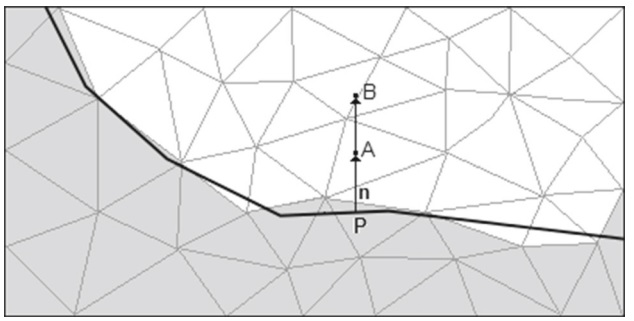
\includegraphics[width=\textwidth]{bajger}
			 \footnotesize (P. Bajger et al. 2017)
			\end{figure}
		\end{column}
	\end{columns}

\end{frame}


\begin{frame}[fragile]{Computational Mesh}

	\begin{columns}[t]
		\begin{column}{.45\textwidth}
		\begin{itemize}
	\item	
Eulerian mesh
\item
Generated using Netgen in SALOME platform
\item
Adaptively refined on the moving interface 
		\end{itemize}
		
		\end{column}
		\begin{column}{.55\textwidth}
			\vspace{-0.8cm}
			\begin{figure}
			\centering
			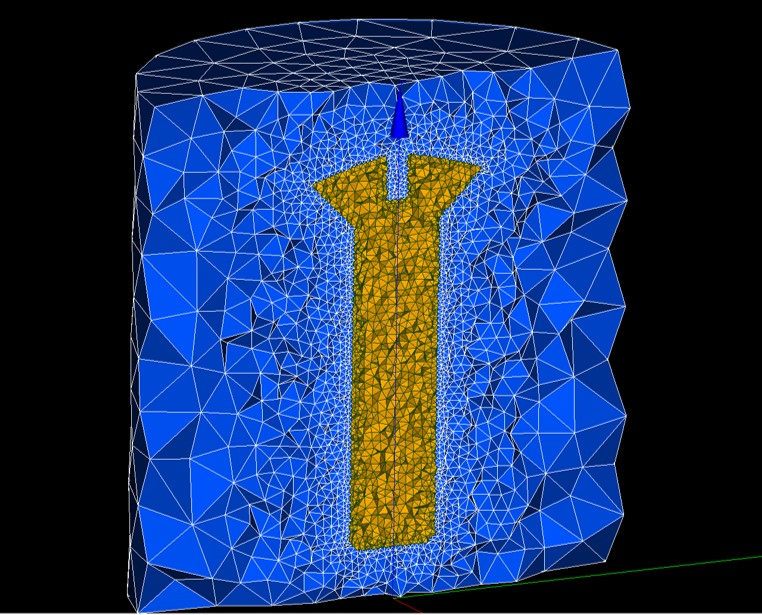
\includegraphics[width=\textwidth]{mesh_screw}

			\end{figure}
		\end{column}
	\end{columns}

\end{frame}


\begin{frame}[fragile]{Parallelization}

\begin{itemize}
\item
Message Passing Interface
\item
Distributed numerical integration\\
(assigning a number in the range of [0, MPI Size-1] to each element)
\item
MUMPS multifrontal direct solver
\end{itemize}

\end{frame}



\section{Simulation Results}

\begin{frame}[fragile]{Release of Ions and Degradation - Simple Screw}

		\begin{figure}
			\centering
			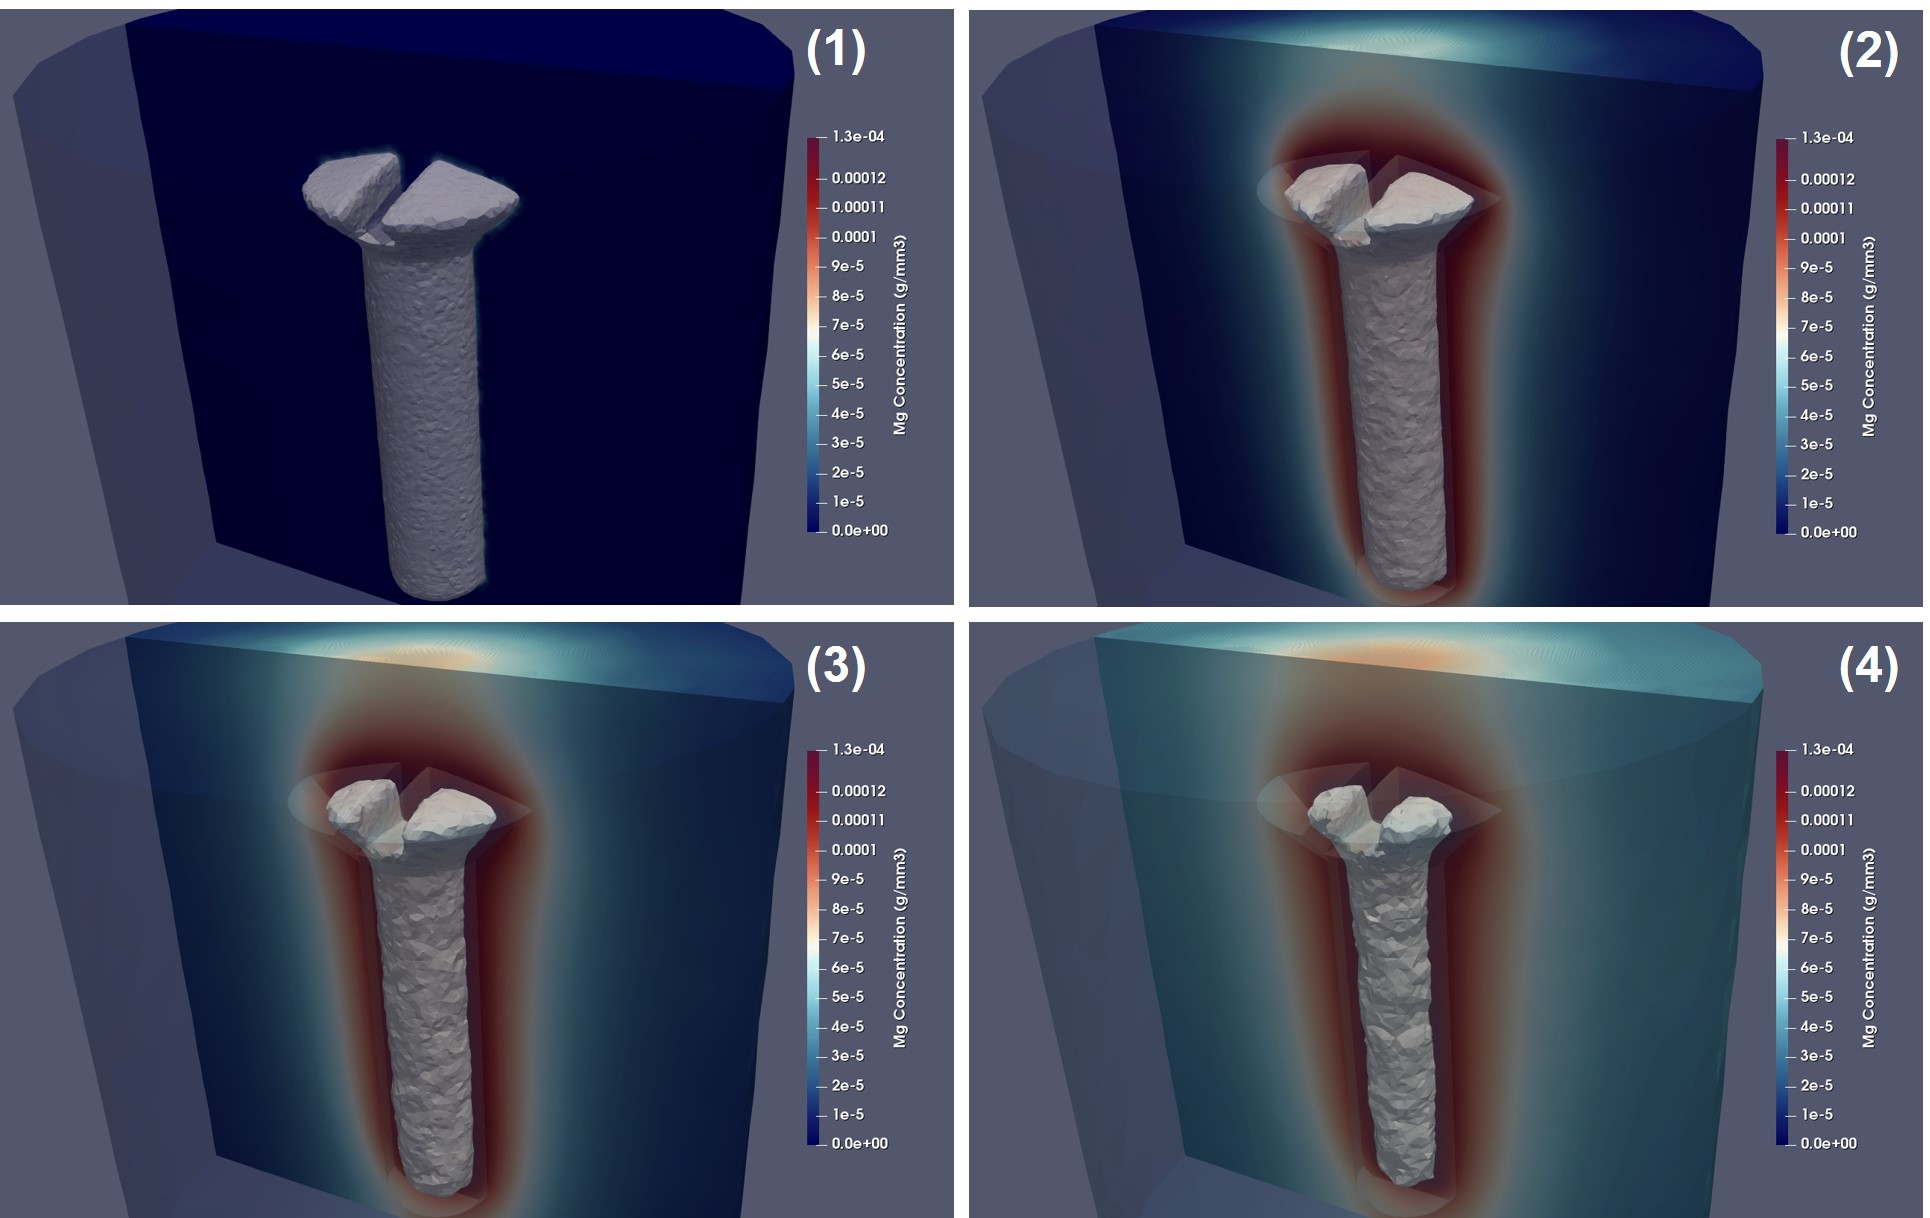
\includegraphics[width=0.7\textwidth] {screw_result}
			
		\end{figure}

\end{frame}


\begin{frame}[fragile]{Film Formation - Simple Screw}

		\begin{figure}
			\centering
			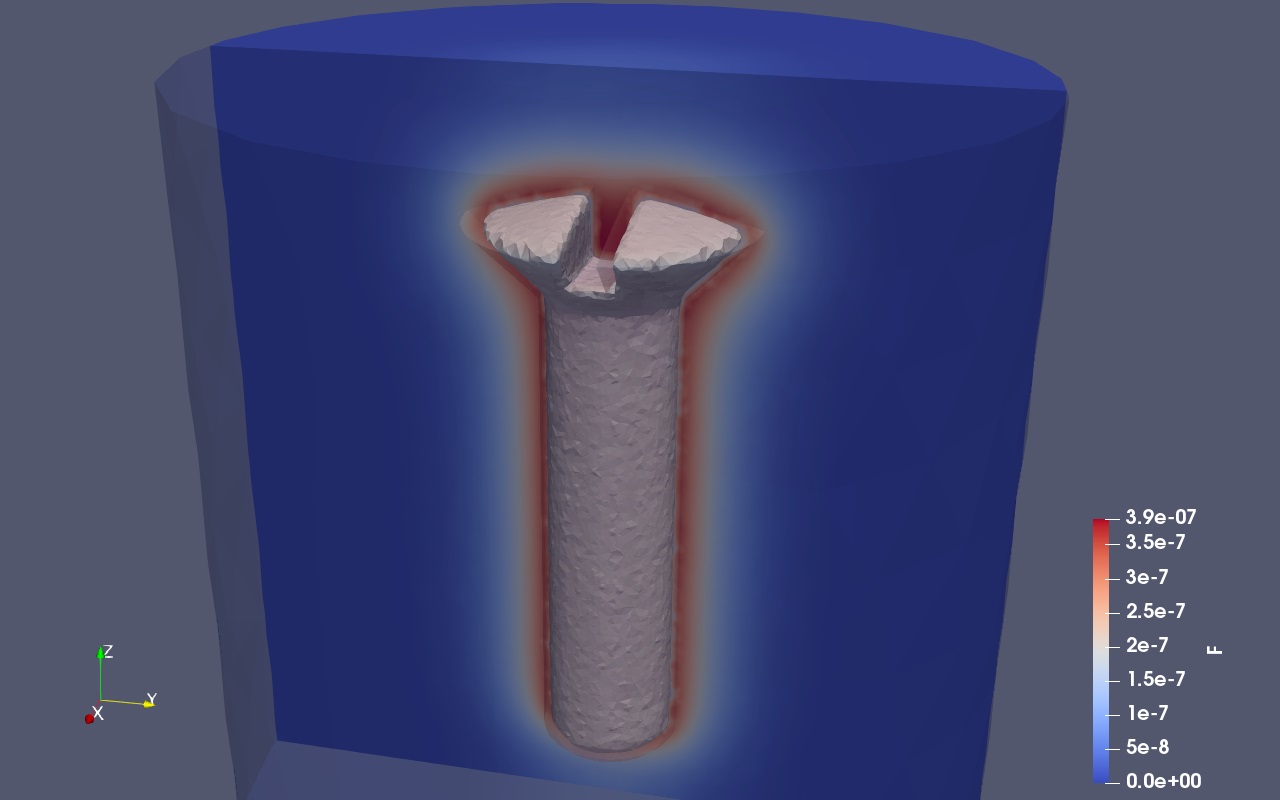
\includegraphics[width=0.5\textwidth] {screw_film}
			
			\footnotesize Formation of the protective film on the interface of material-medium
			
		\end{figure}

\end{frame}


\begin{frame}[fragile]{Release of Ions and Degradation - Porous Structure}

	\begin{columns}[t]
		\begin{column}{.50\textwidth}
			\begin{figure}
			\centering
			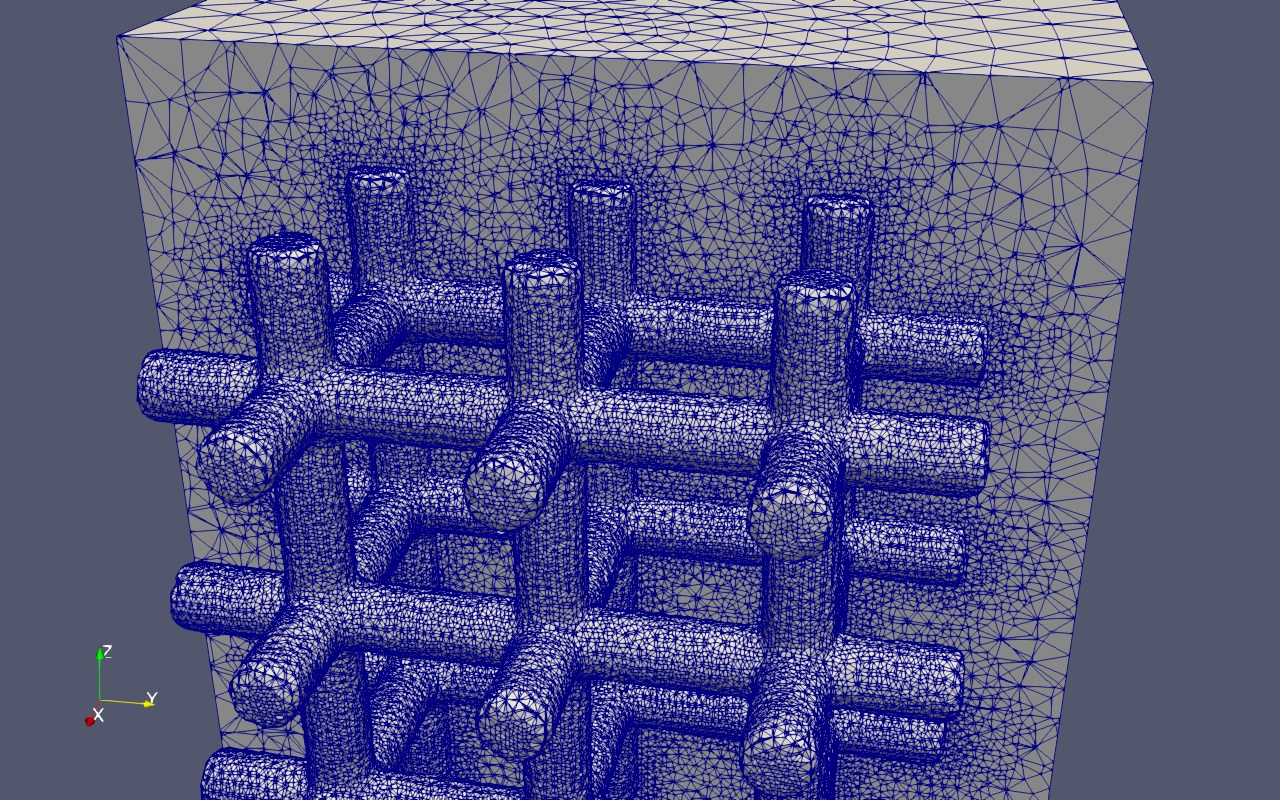
\includegraphics[width=\textwidth]{porous_mesh}
			
			\footnotesize	Trimmed view of the computational mesh
			\end{figure}
		\end{column}
		\begin{column}{.50\textwidth}

			\begin{figure}
			\centering
			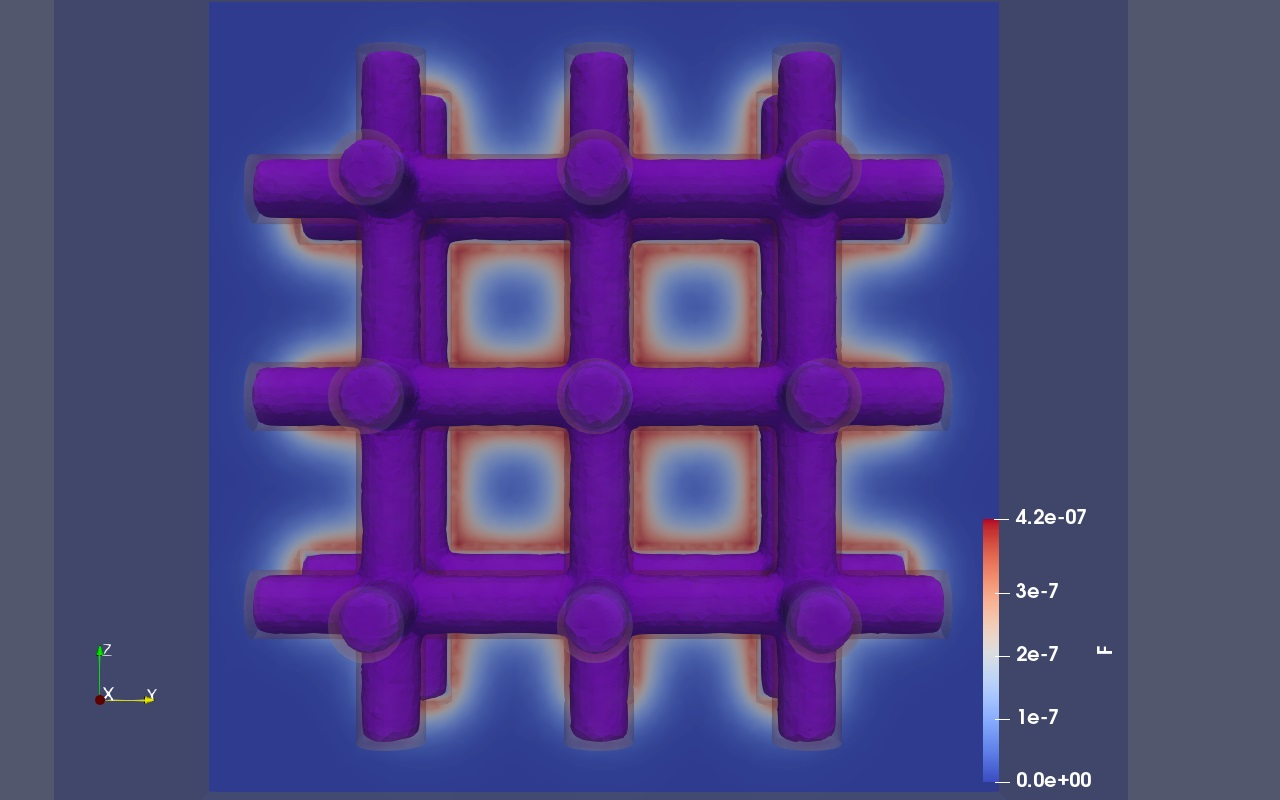
\includegraphics[width=\textwidth]{porous_film}
			
			\footnotesize	Formation of the protective film
			\end{figure}
		\end{column}
	\end{columns}



\end{frame}

\begin{frame}[fragile]{Quantitative Results}

	\begin{columns}[t]
		\begin{column}{.65\textwidth}
			Measuring mass loss:
			\begin{itemize}
			\item
			Direct weight reduction
			\item
			Side products evolution
			\end{itemize}
			
		Using level set output for calculating mass loss
			\begin{gather*}
			\mathrm{Mg}_{\mathrm{lost}}=\int_{\Omega_{+}(t)} \mathrm{Mg}_{\mathrm{solid}} \mathrm{d} V-\int_{\Omega_{+}(0)} \mathrm{Mg}_{\mathrm{solid}} \mathrm{d} V_{0}
			\end{gather*}		
			\begin{gather*}
			\Omega_{+}(t)=\{\mathbf{x}: \phi(\mathbf{x}, t) \geq 0\}
			\end{gather*}
		\end{column}
		\begin{column}{.35\textwidth}
			\vspace{-2cm}
			\begin{figure}
			\centering
			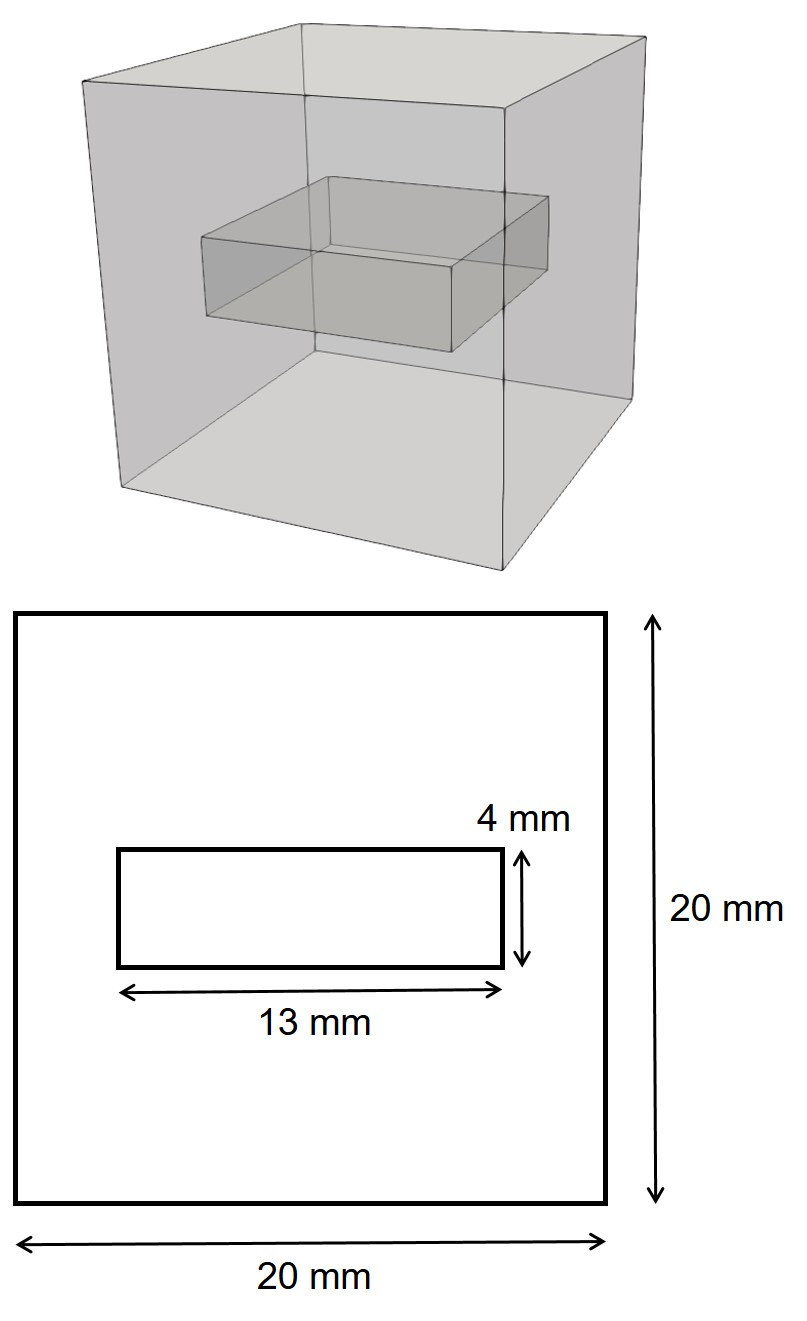
\includegraphics[width=0.9\textwidth]{simulation_setup}
			
			\footnotesize	Simulation and experimental setup 
			\end{figure}
		\end{column}
	\end{columns}

\end{frame}


\begin{frame}[fragile]{Mass Loss and Evolving Side Products}

		\begin{figure}
			\centering
			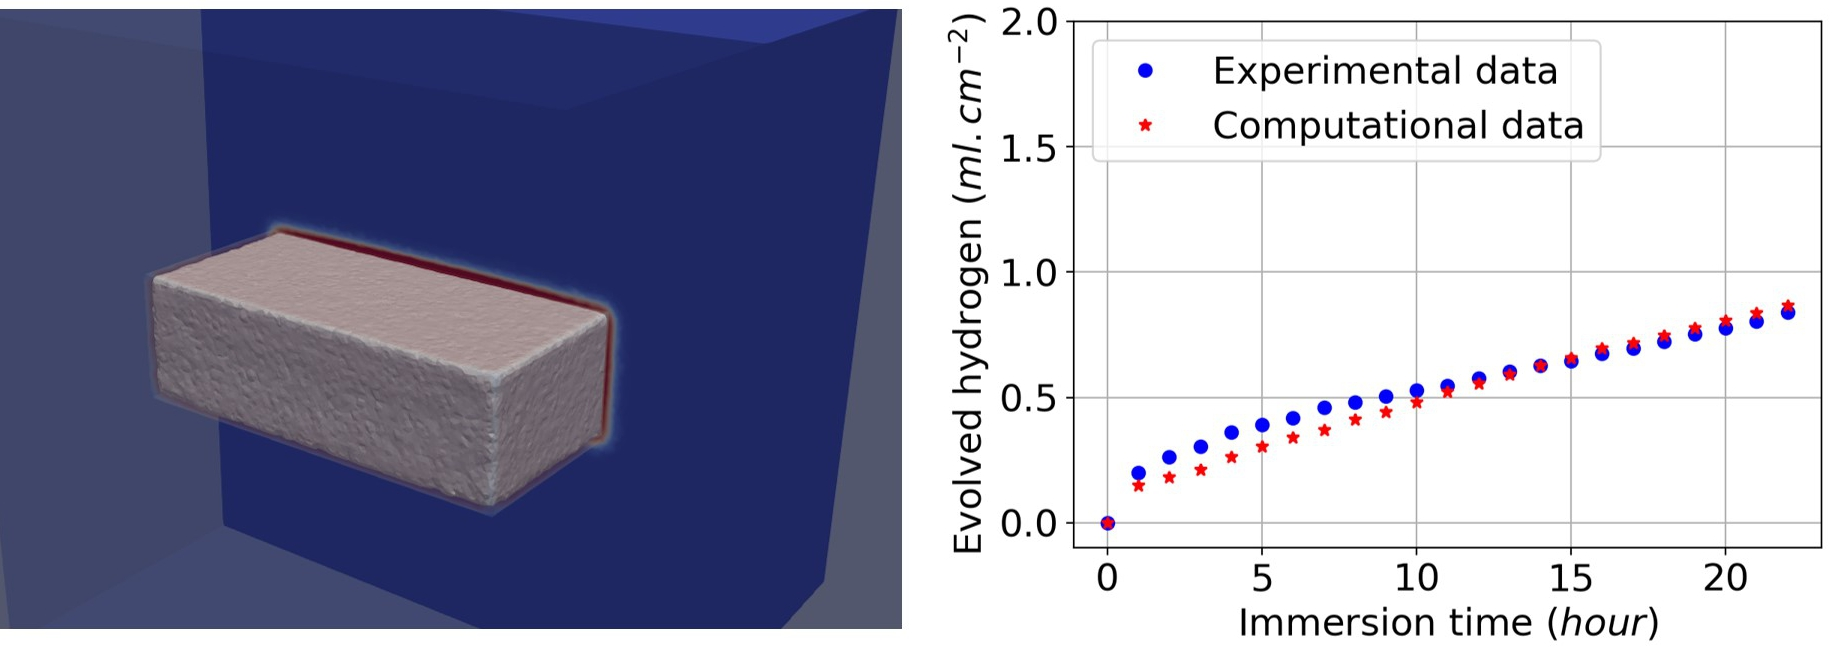
\includegraphics[width=0.8\textwidth] {numerical_results}
			
			\footnotesize Film formation and the comparison of predicted and experimental mass loss, measured by the evolved hydrogen gas
			
			
		\end{figure}

\end{frame}


\section{Performance Analysis}


\begin{frame}[fragile]{Problem Size}  

\begin{itemize}
\item
Same setup as the model for calibration and validation
\item
DOF: 144k
\item
Elements: 831k (P1)
\end{itemize}

	\begin{figure}
			\centering
			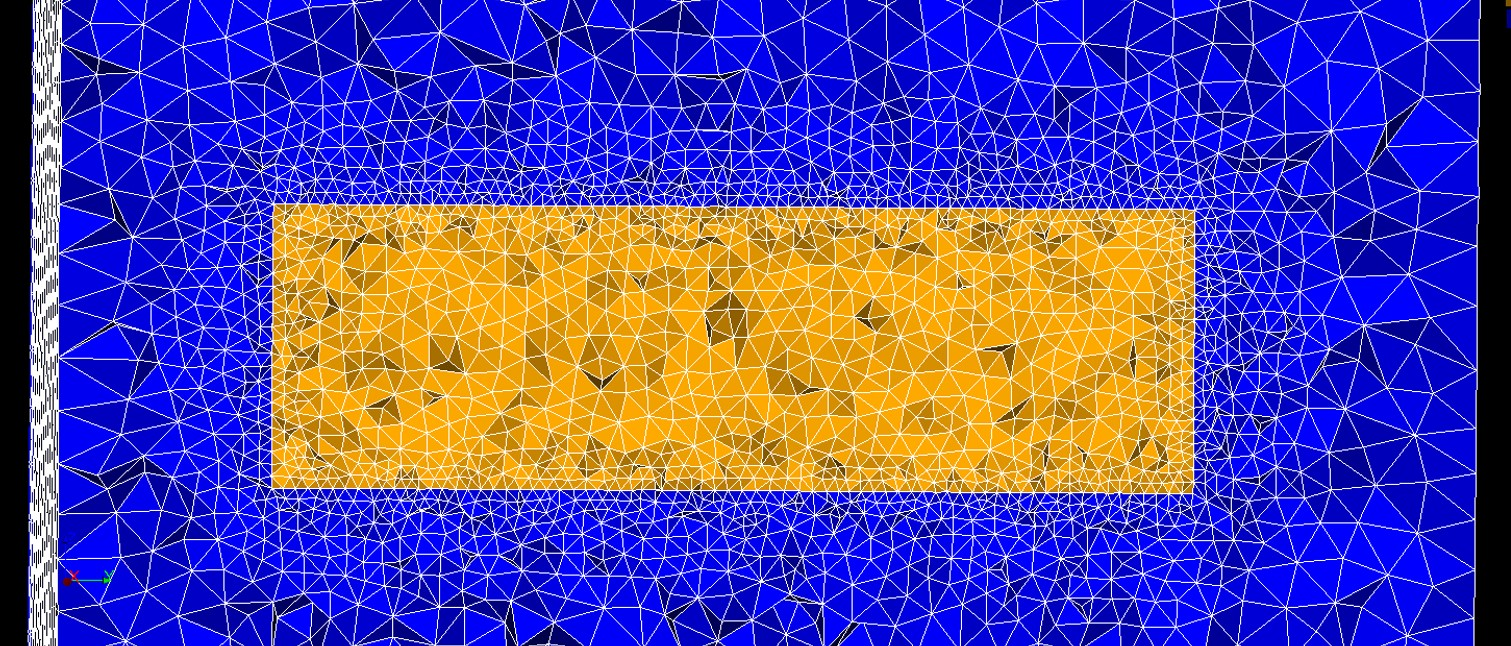
\includegraphics[width=0.7\textwidth]{mesh}
			 
	\end{figure}

\end{frame}


\begin{frame}[fragile]{Domain Decomposition}

	\begin{columns}[t]
		\begin{column}{.50\textwidth}
			\begin{figure}
			\centering
			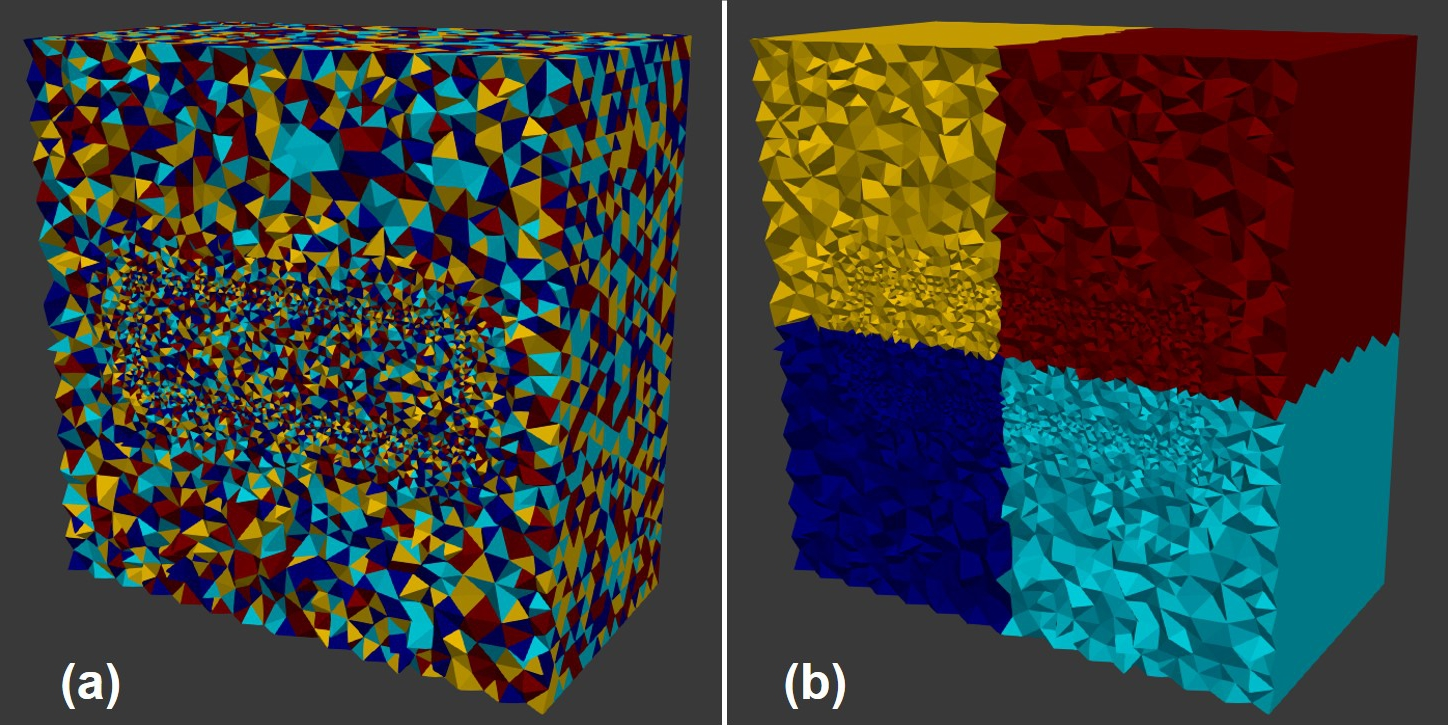
\includegraphics[width=\textwidth]{domain_decomp_mesh}
			
			\footnotesize	Two different approaches for domain decomposition. Colors show different mesh regions assigned to different MPI cores.
			\end{figure}
		\end{column}
		\begin{column}{.50\textwidth}

			\begin{figure}
			\centering
			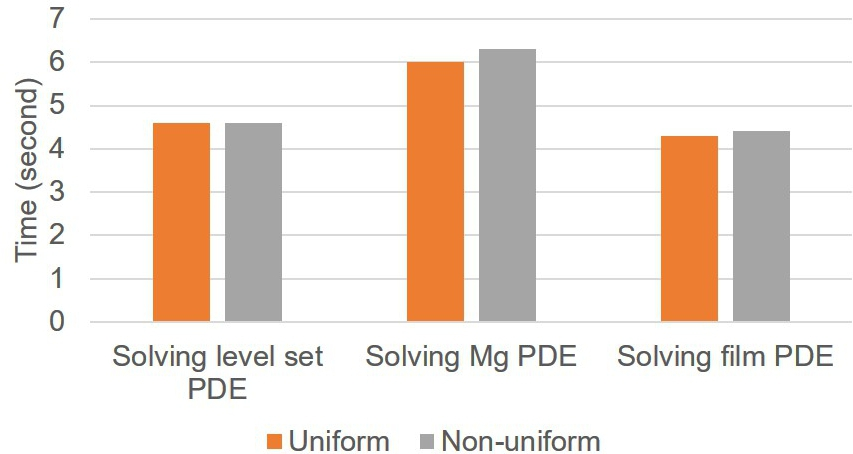
\includegraphics[width=\textwidth]{domain_decomp_result}
			
			\footnotesize	Execution time per time step 
			\end{figure}
		\end{column}
	\end{columns}	
	


\end{frame}


\begin{frame}[fragile]{Weak-Scaling Test Results}
	
\begin{figure}
	\centering
	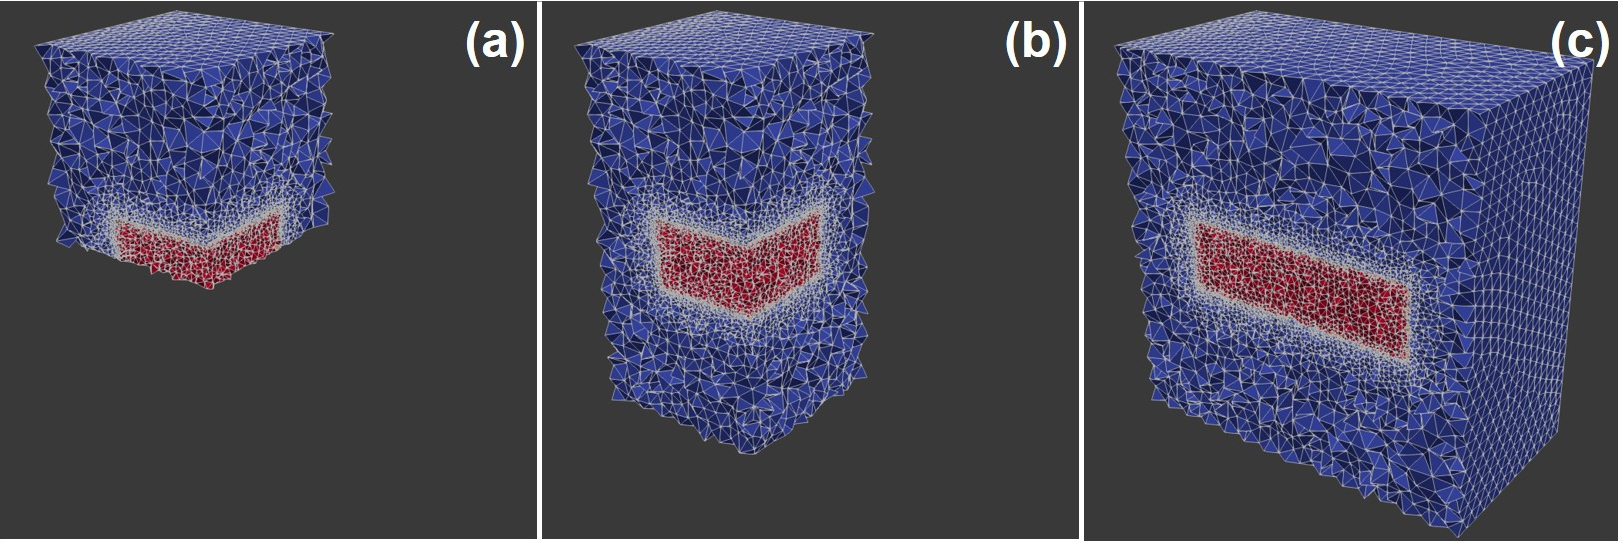
\includegraphics[width=0.5\textwidth]{weak_scaling_models}
	
	
	\end{figure}
	
	
	\begin{figure}
	\centering
	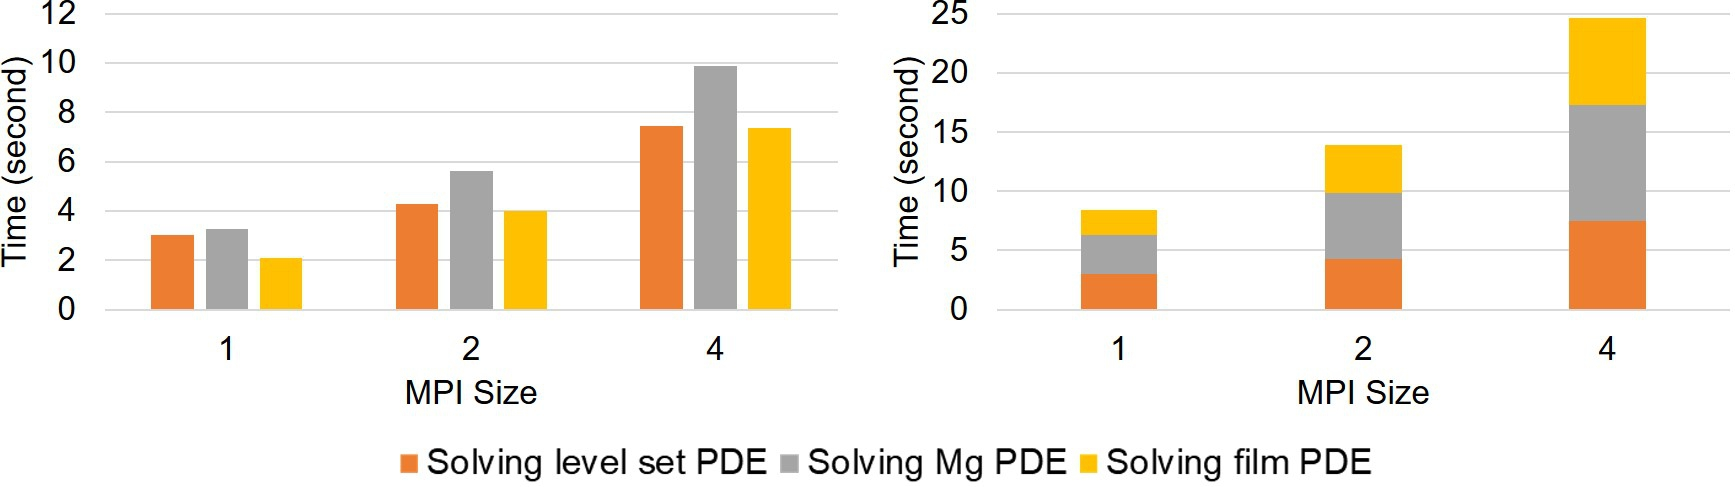
\includegraphics[width=0.7\textwidth]{weak_scaling_results}
	
	\end{figure}
	

\end{frame}


\begin{frame}[fragile]{Weak-Scaling Test Analysis}

Based on Gustafson’s law:
\begin{gather*}
\mathrm{Speedup} = f + (1-f) \times N
\end{gather*}

Serial proportion = 86\%, Parallelizable proportion = 14\%

	\begin{figure}
			\centering
			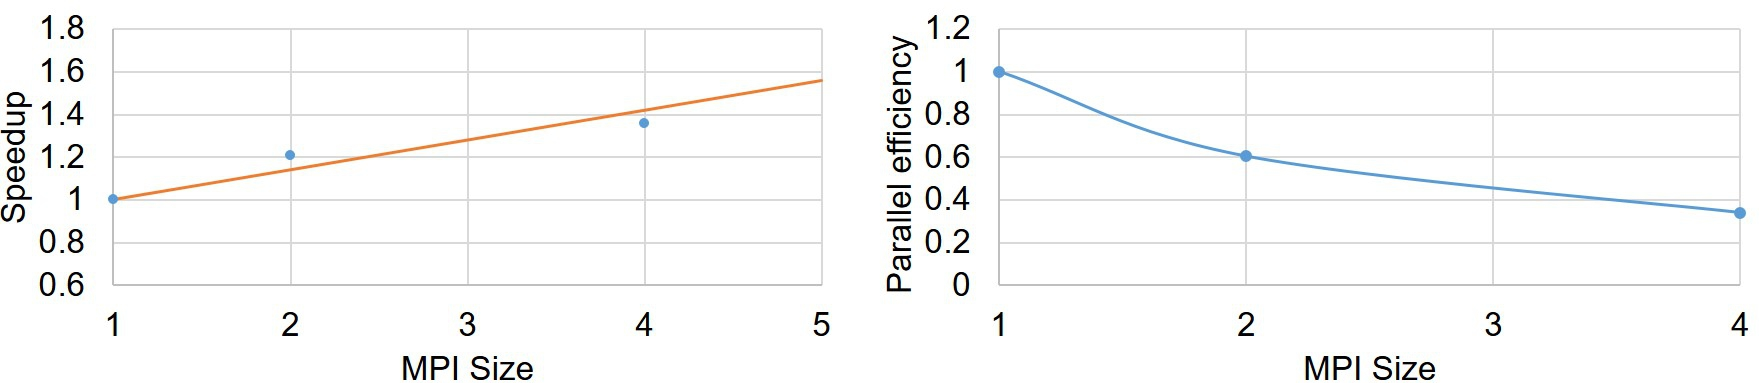
\includegraphics[width=0.8\textwidth]{weak_scaling_analysis}
			
	\end{figure}


\end{frame}


\begin{frame}[fragile]{Strong-Scaling Test Results}

	\vspace{1cm}
	
	\begin{figure}
	\centering
	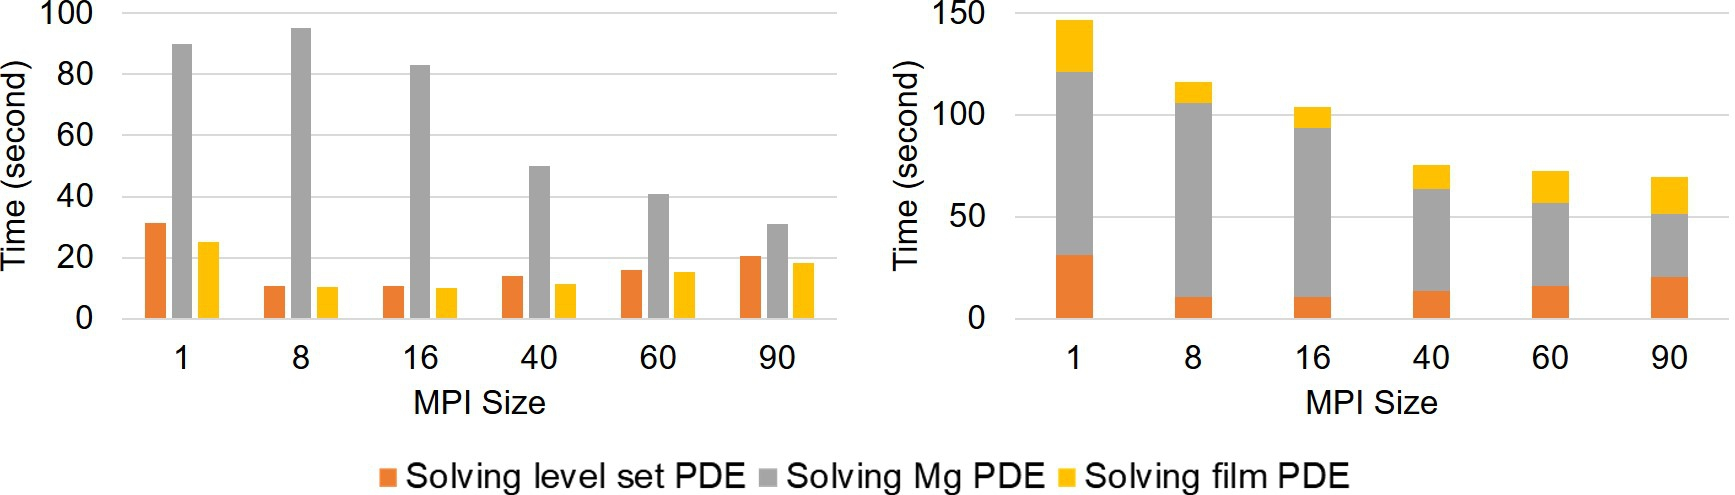
\includegraphics[width=0.9\textwidth]{strong_scaling_results}
	
	\footnotesize Time required to solve each PDE in each time step
	
	\end{figure}

\end{frame}

\begin{frame}[fragile]{Strong-Scaling Test Analysis}

Based on Amdahl's law:
\begin{gather*}
\mathrm{Speedup} = \frac{1}{f + \frac{1-f}{N}}
\end{gather*}

Serial proportion = 52\%, Parallelizable proportion = 48\%
	\begin{figure}
			\centering
			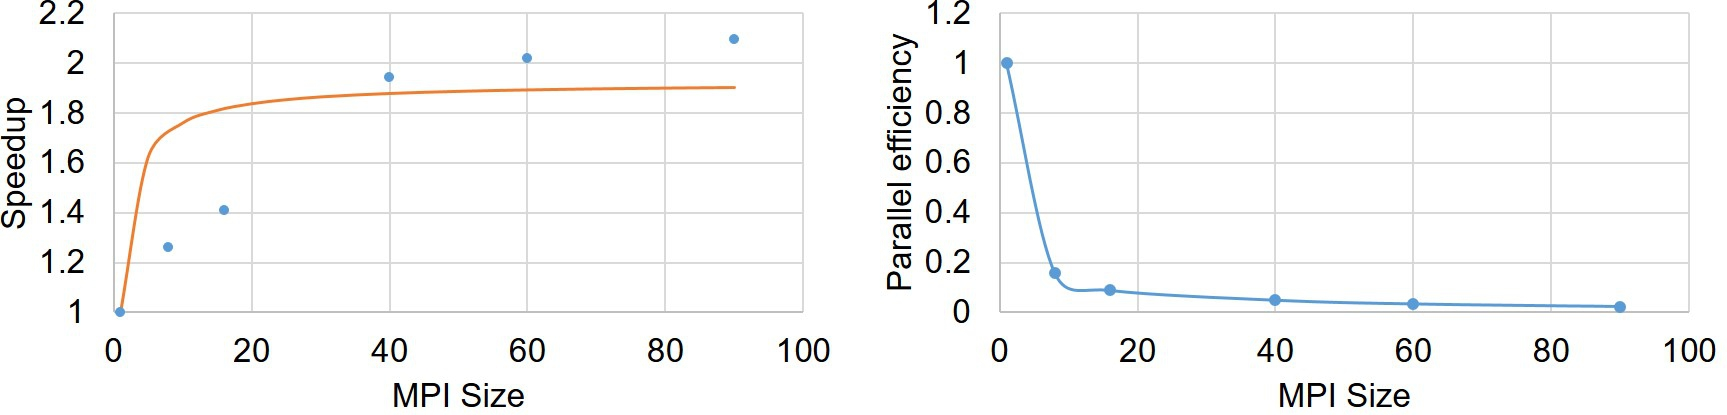
\includegraphics[width=0.8\textwidth]{strong_scaling_analysis}
			
	\end{figure}
	


\end{frame}



\begin{frame}[fragile]{Conclusion}

\begin{itemize}
\item
A quantitative mathematical model and its corresponding computational model to assess the degradation behavior of biodegradable materials
\item 
Using level set method to track the moving corrosion front during degradation
\item
Once fully validated, the model will be an important tool to find the right design and properties of the metallic biomaterials and implants

\end{itemize}
	


\end{frame}


\begin{frame}[c,plain,noframenumbering]
\begin{tikzpicture}[remember picture,overlay]
\fill[fill=kul-blue]
    (current page.south east)  rectangle  ([shift={(0,-0.1\paperheight)}]current page.north west)   ;
\end{tikzpicture}

\centering
\textcolor{white}{\huge Thank you for your attention}

\vspace{2cm}

{\large mojtaba.barzegari@kuleuven.be}
\end{frame}

\end{document}
